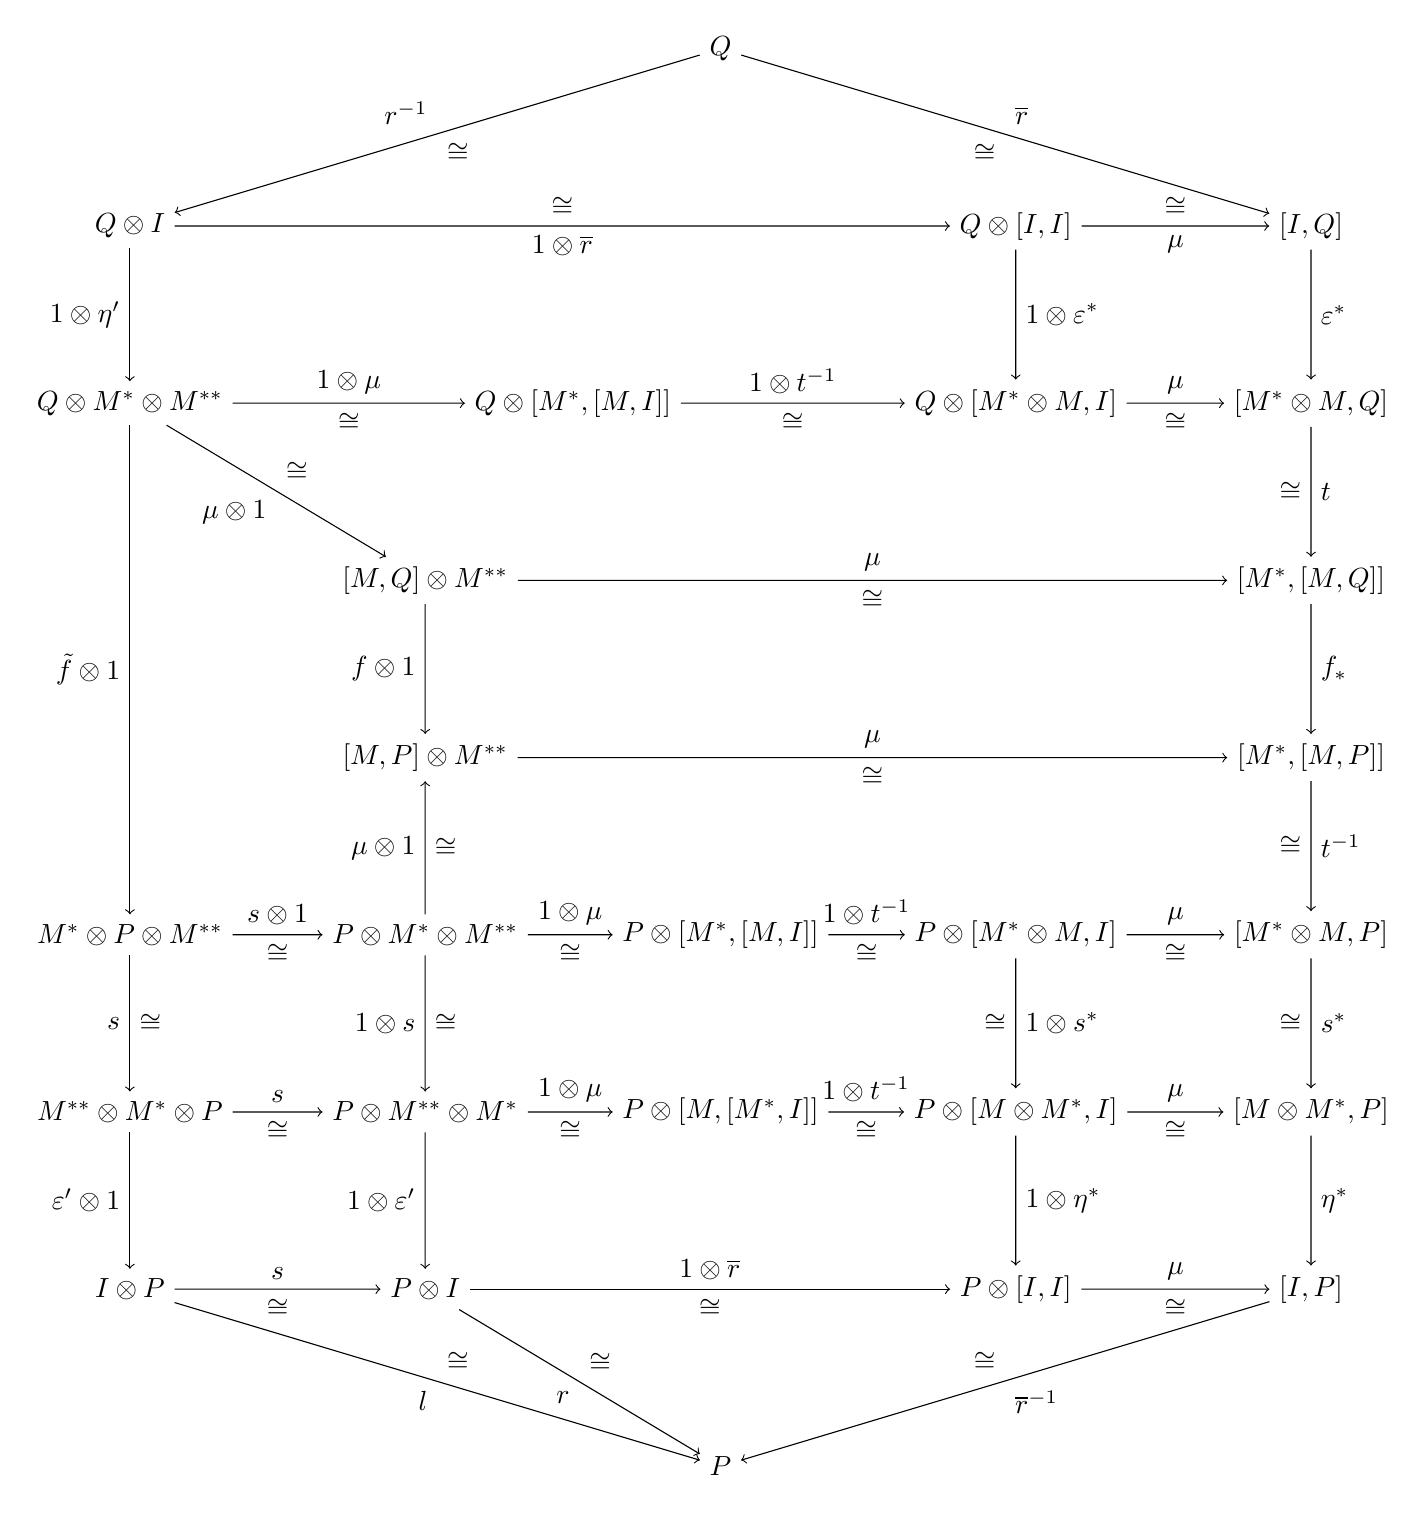
\begin{tikzpicture}[xscale=3.75, yscale=2.25]
	\node(A) at (2, 8){$Q$};
	\node(B) at (0, 7){$Q \otimes I$};
	\node(C) at (3, 7){$Q \otimes \left[I, I\right]$};
	\node(D) at (4, 7){$\left[I, Q\right]$};
	\node(E) at (0, 6){$Q \otimes M^* \otimes M^{**}$};
	\node(F) at (1.5, 6){$Q \otimes \left[M^*, \left[M, I\right]\right]$};
	\node(G) at (3, 6){$Q \otimes \left[M^* \otimes M, I\right]$};
	\node(H) at (4, 6){$\left[M^* \otimes M, Q\right]$};
	\node(I) at (1, 5){$\left[M, Q\right] \otimes M^{**}$};
	\node(J) at (4, 5){$\left[M^*, \left[M, Q\right]\right]$};
	\node(M) at (1, 4){$\left[M, P\right] \otimes M^{**}$};
	\node(N) at (4, 4){$\left[M^*, \left[M, P\right]\right]$};
	\node(K) at (0, 3){$M^* \otimes P \otimes M^{**}$};
	\node(L) at (1, 3){$P \otimes M^* \otimes M^{**}$};
	\node(O) at (2, 3){$P \otimes \left[M^*, \left[M, I\right]\right]$};
	\node(P) at (3, 3){$P \otimes \left[M^* \otimes M, I\right]$};
	\node(Q) at (4, 3){$\left[M^* \otimes M, P\right]$};
	\node(R) at (0, 2){$M^{**} \otimes M^* \otimes P$};
	\node(S) at (1, 2){$P \otimes M^{**} \otimes M^*$};
	\node(T) at (2, 2){$P \otimes \left[M, \left[M^*, I\right]\right]$};
	\node(U) at (3, 2){$P \otimes \left[M \otimes M^*, I\right]$};
	\node(V) at (4, 2){$\left[M \otimes M^*, P\right]$};
	\node(W) at (0, 1){$I \otimes P$};
	\node(X) at (1, 1){$P \otimes I$};
	\node(Y) at (3, 1){$P \otimes \left[I, I\right]$};
	\node(Z) at (4, 1){$\left[I, P\right]$};
	\node(A1) at (2, 0){$P$};


	\draw [->] (A) -- node[above left]{$r^{-1}$} node[below right]{$\cong$} (B);
	\draw [->] (A) -- node[above right]{$\overline{r}$} node[below left]{$\cong$} (D);
	\draw [->] (B) -- node[below]{$1 \otimes \overline{r}$} node[above]{$\cong$} (C);
	\draw [->] (C) -- node[below]{$\mu$} node[above]{$\cong$} (D);
	\draw [->] (B) -- node[left]{$1 \otimes \eta'$} (E);
	\draw [->] (E) -- node[above]{$1 \otimes \mu$} node[below]{$\cong$} (F);
	\draw [->] (F) -- node[above]{$1 \otimes t^{-1}$} node[below]{$\cong$} (G);
	\draw [->] (C) -- node[right]{$1 \otimes \varepsilon^*$} (G);
	\draw [->] (G) -- node[above]{$\mu$} node[below]{$\cong$} (H);
	\draw [->] (D) -- node[right]{$\varepsilon^*$} (H);
	\draw [->] (E) -- node[below left]{$\mu \otimes 1$} node[above right]{$\cong$} (I);
	\draw [->] (I) -- node[above]{$\mu$} node[below]{$\cong$} (J);
	\draw [->] (H) -- node[right]{$t$} node[left]{$\cong$} (J);
	\draw [->] (E) -- node[left]{$\tilde{f} \otimes 1$} (K);
	\draw [->] (K) -- node[above]{$s \otimes 1$} node[below]{$\cong$} (L);
	\draw [->] (L) -- node[left]{$\mu \otimes 1$} node[right]{$\cong$} (M);
	\draw [->] (I) -- node[left]{$f \otimes 1$} (M);
	\draw [->] (M) -- node[above]{$\mu$} node[below]{$\cong$} (N);
	\draw [->] (J) -- node[right]{$f_*$} (N);
	\draw [->] (K) -- node[left]{$s$} node[right]{$\cong$} (R);
	\draw [->] (R) -- node[above]{$s$} node[below]{$\cong$} (S);
	\draw [->] (L) -- node[left]{$1 \otimes s$} node[right]{$\cong$} (S);
	\draw [->] (L) -- node[above]{$1 \otimes \mu$} node[below]{$\cong$} (O);
	\draw [->] (O) -- node[above]{$1 \otimes t^{-1}$} node[below]{$\cong$} (P);
	\draw [->] (P) -- node[above]{$\mu$} node[below]{$\cong$} (Q);
	\draw [->] (N) -- node[right]{$t^{-1}$} node[left]{$\cong$} (Q);
	\draw [->] (S) -- node[above]{$1 \otimes \mu$} node[below]{$\cong$} (T);
	\draw [->] (T) -- node[above]{$1 \otimes t^{-1}$} node[below]{$\cong$} (U);
	\draw [->] (P) -- node[right]{$1 \otimes s^*$} node[left]{$\cong$} (U);
	\draw [->] (U) -- node[above]{$\mu$} node[below]{$\cong$} (V);
	\draw [->] (Q) -- node[right]{$s^*$} node[left]{$\cong$} (V);
	\draw [->] (R) -- node[left]{$\varepsilon' \otimes 1$} (W);
	\draw [->] (W) -- node[above]{$s$} node[below]{$\cong$} (X);
	\draw [->] (S) -- node[left]{$1 \otimes \varepsilon'$} (X);
	\draw [->] (X) -- node[above]{$1 \otimes \overline{r}$} node[below]{$\cong$} (Y);
	\draw [->] (U) -- node[right]{$1 \otimes \eta^*$} (Y);
	\draw [->] (Y) -- node[above]{$\mu$} node[below]{$\cong$} (Z);
	\draw [->] (V) -- node[right]{$\eta^*$} (Z);
	\draw [->] (W) -- node[below left]{$l$} node[above right]{$\cong$} (A1);
	\draw [->] (X) -- node[below left]{$r$} node[above right]{$\cong$} (A1);
	\draw [->] (Z) -- node[below right]{$\overline{r}^{-1}$} node[above left]{$\cong$} (A1);
\end{tikzpicture}
